\paragraph{Scenarios}
\begin{enumerate}
    \item Henry is a member of the local police of the city of Casalpusterlengo, a municipality that has a partnership with SafeStreets. Every month he wants to check the most unsafe areas in the city, so that he could better patrol the city. This could be done by opening the SafeStreets app and selecting "analyze" tab, then selecting the violation density map option and using the previous month as temporal filter.
    
    \item Lucia, a worker of Bergamo's municipality, is interested in studying possible solutions to recurrent parking violations along Via Milano. Bergamo's municipality is regularly registered to SafeStreets system, so she decides to try to check the list of interventions suggested from SafeStreets' algorithm. After she log in the app, she just need to check the suggestions tab to search for valid ones in that area, then she can also rate them to improve the suggestion system.
\end{enumerate}

\begin{figure}[H]
        \centering
        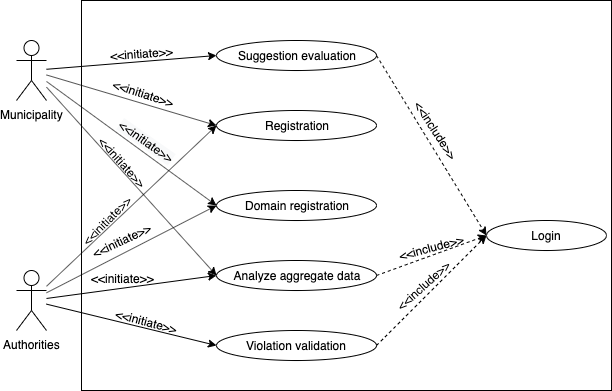
\includegraphics[width=\textwidth]{UML/UseCaseThirdParty}
\end{figure}

\vskip 0.2in
\begin{tabular}{|p{3.1cm}|p{11.6cm}|}
\hline
Name & Login\\
\hline
Actors & Authorities and municipality\\
\hline
Entry Condition & The actor opens the app.\\
\hline
Event flow & \begin{enumerate}
                \item The actor inserts his email.
                \item The actor inserts his password.
                \item The actor press the login button.
            \end{enumerate}\\
\hline
Exit condition & The actor is authenticated and login is successful.\\
\hline
Exception & Username or password are invalid, "invalid credentials" message is displayed and the actor needs to insert credentials again.\\
\hline
\end{tabular}

\vskip 0.2in
\begin{tabular}{|p{3.1cm}|p{11.6cm}|}
\hline
Name & Registration\\
\hline
Actors & Authorities or municipalities\\
\hline
Entry Condition & An authority or municipality opens the app and has no valid account\\
\hline
Event flow & \begin{enumerate}
                \item The actor inserts the desired username.
                \item The actor inserts the desired password.
                \item The actor confirms his password.
                \item The actor inserts his official public certified email (PCE) given for his public office.
                \item The actor inserts his birthday.
                \item The system checks the authenticity of the the email using its domain.
            \end{enumerate}\\
\hline
Exit condition & The email is authenticated and the user is redirected to login form.\\
\hline
Exception & Email is already in use, or is not a PEC email, or confirm password field content diverge from password, in this case the user is alerted with a proper message on screen and asked to correct the data.\\
\hline
\end{tabular}

\vskip 0.2in
\begin{tabular}{|p{3.1cm}|p{11.6cm}|}
\hline
Name & Analyze aggregate data\\
\hline
Actors & Authorities\\
\hline
Entry Condition & The Actor wants to know some information about the reported violations.\\
\hline
Event flow & \begin{enumerate}
                \item The Actor selects the "aggregated data" tab.
                \item The Actor selects the topic he/she is interested about.
                \item The Actor may select an appropriate filter for his search.
                \item The Actor selects the data of interest.
                \item The system provides the data to be visualized according to the actor's authorization level.
                \item The Actor visualizes the data.
            \end{enumerate}\\
\hline
Exit condition & The Actor finishes to analyze the data.\\
\hline
\end{tabular}

\vskip 0.2in
\begin{tabular}{|p{3.1cm}|p{11.6cm}|}
\hline
Name & Violation convalidation\\
\hline
Actors & Authorities\\
\hline
Entry Condition & A report is received by the authorities.\\
\hline
Event flow & \begin{enumerate}
                \item The authorities check whether the reported violation is an actual traffic violation.
                \item The authorities send a result response (rejected or accepted) to SafeStreets.
                \item The system updates the report status of the violation for the reporting user.
                \item The system augments its data with the reported violation if and only if it was certified by the authorities.
            \end{enumerate}\\
\hline
Exit condition & The violation report and the system violation data are updated.\\
\hline
\end{tabular}

\vskip 0.2in
\begin{tabular}{|p{3.1cm}|p{11.6cm}|}
\hline
Name & Suggestion evaluation\\
\hline
Actors & Municipality\\
\hline
Entry Condition & A municipality is registered on the application and wants to evaluate possible suggested interventions.\\
\hline
Event flow & \begin{enumerate}
			\item The municipality selects the intervention suggestion tab.
			\item The municipality reads and analyzes a list of suggestions.
			\item The municipality chooses and approves zero or more interventions from the list.
            \end{enumerate}\\
\hline
Exit condition & The municipality closes the intervention suggestion tab.\\
\hline
\end{tabular}

% sequence diagrams
\newpage
\textbf{Sequence diagrams}
\begin{figure}[H]
	\centering
	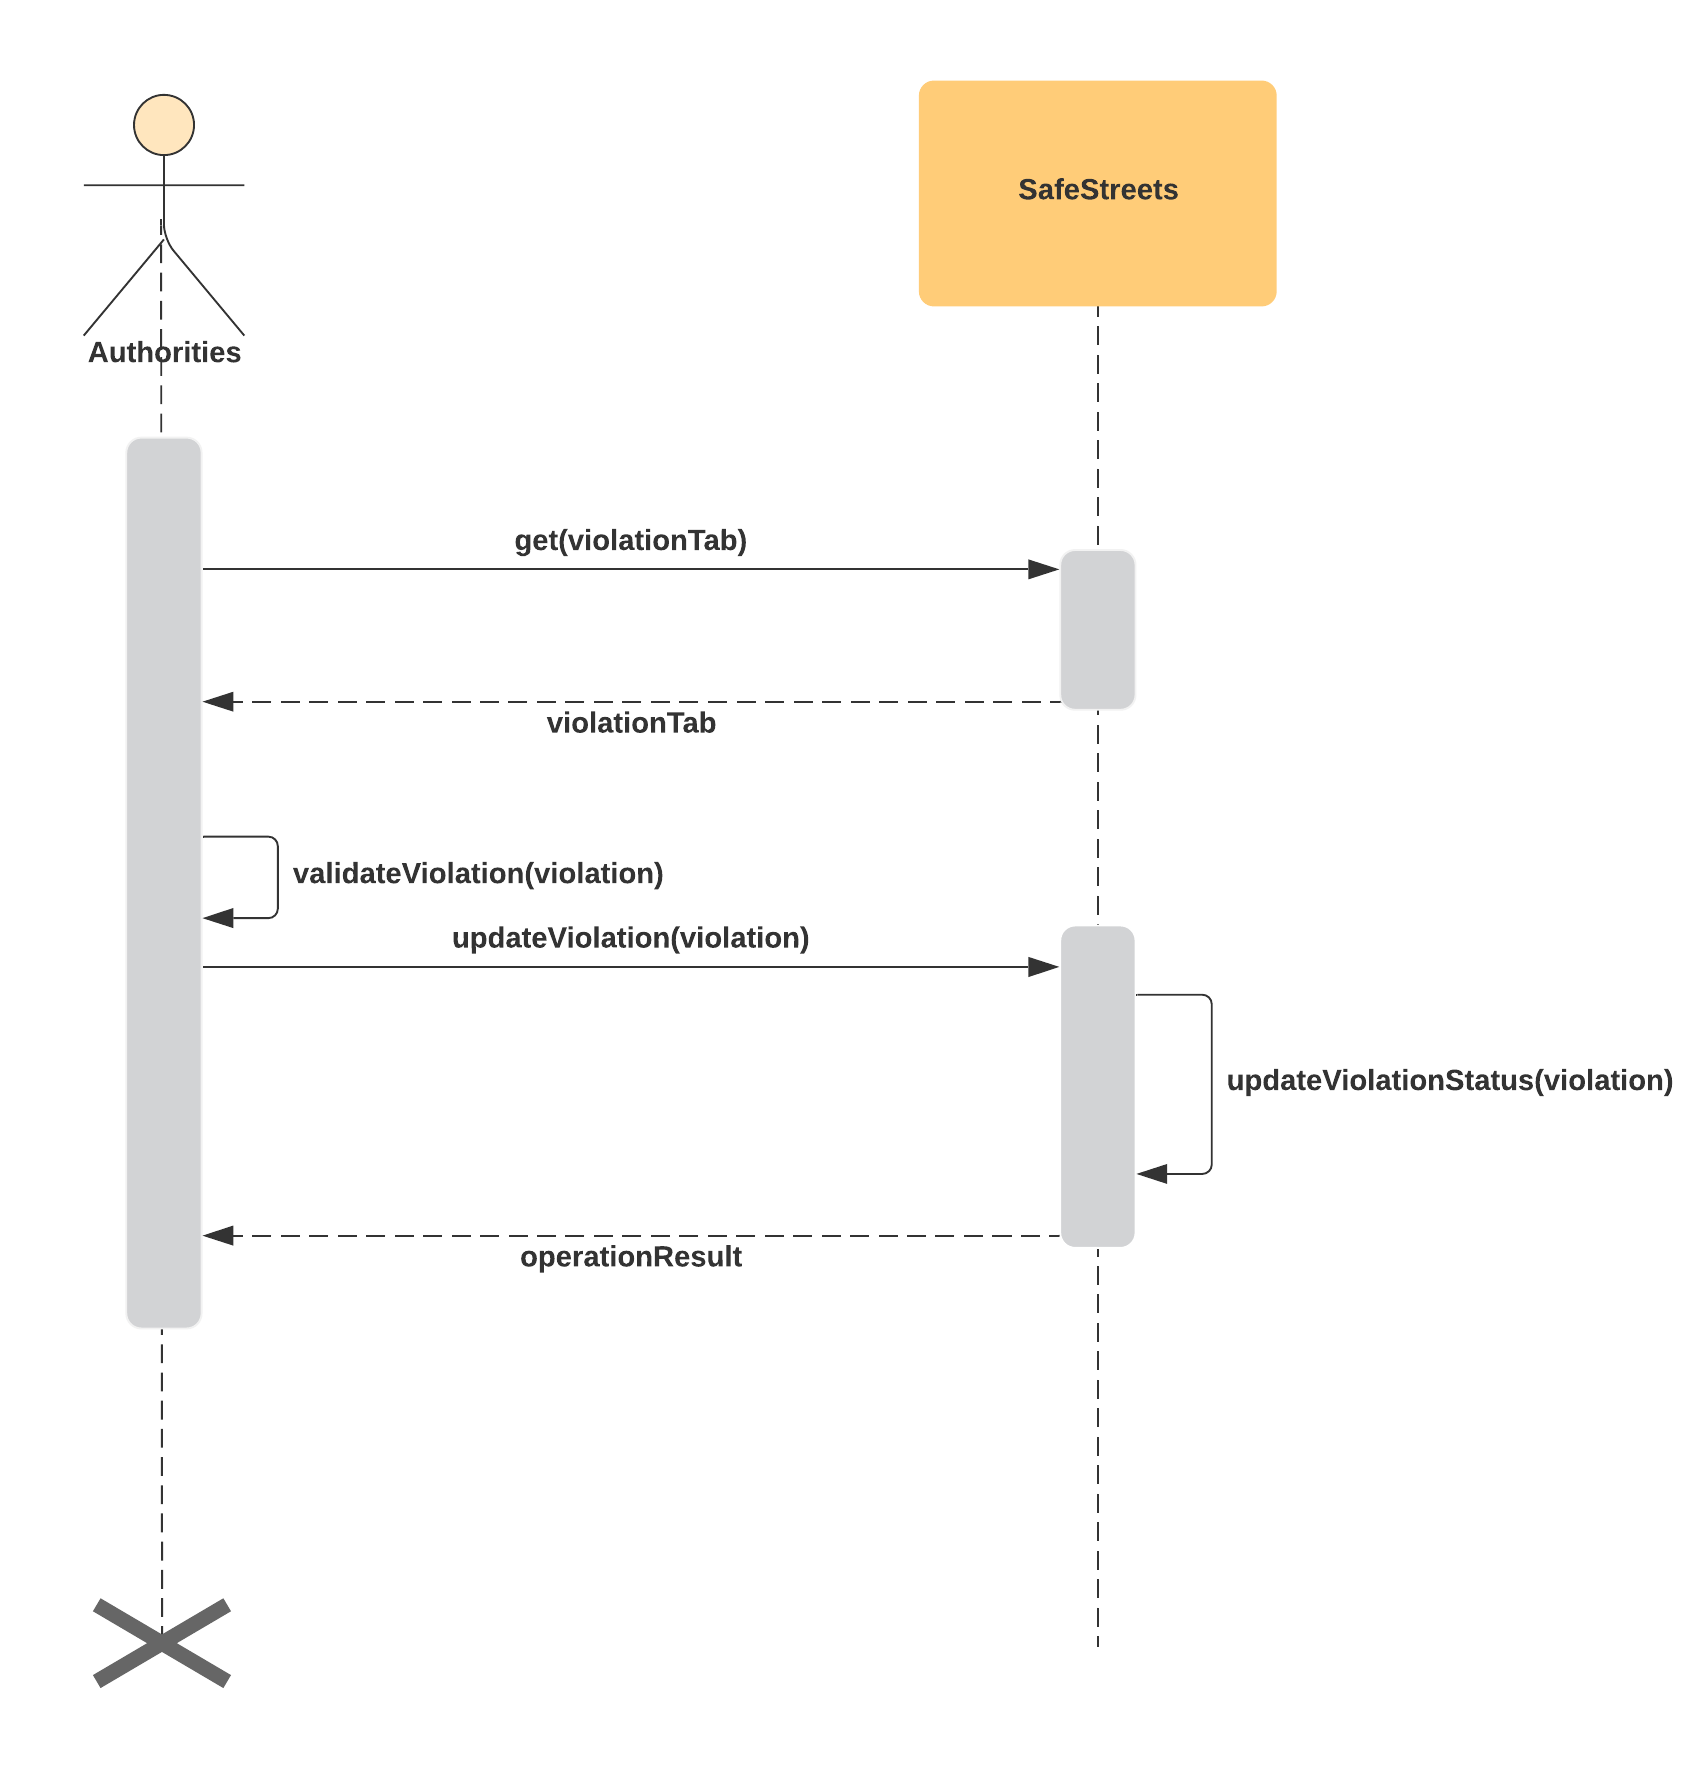
\includegraphics[width=\linewidth]{Images/UML/ViolationValidationUseCase}
	\caption{Violation validation use case.}
\end{figure}
\begin{figure}[H]
	\centering
	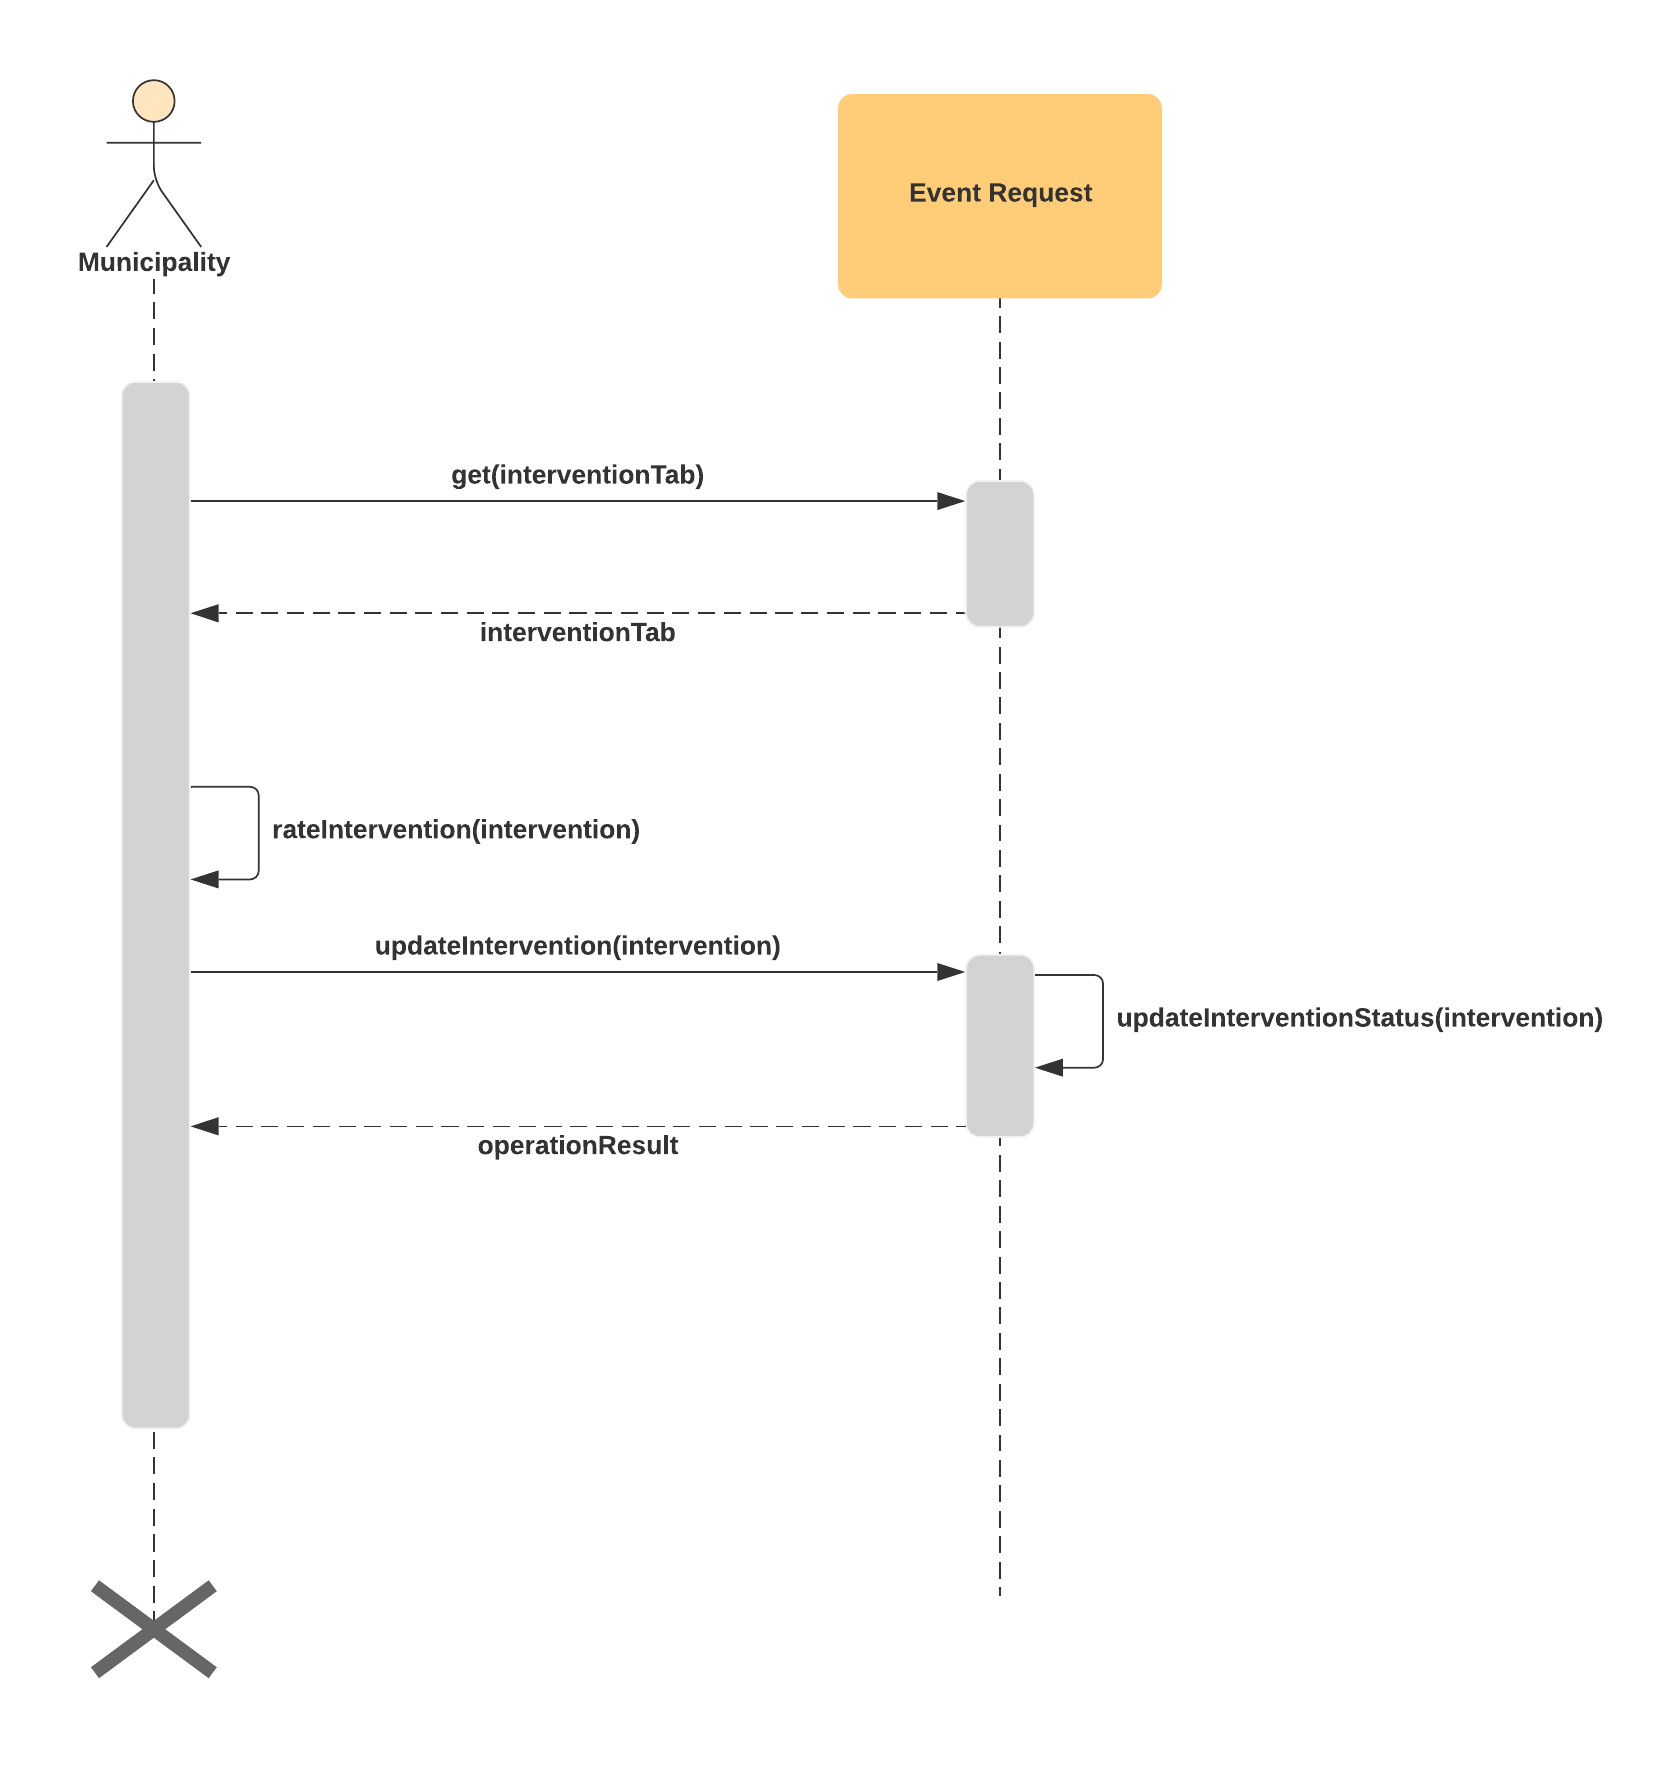
\includegraphics[width=\linewidth]{Images/UML/SuggestionEvaluationUseCase}
	\caption{Suggestion evaluation use case.}
\end{figure}
